\documentclass[tikz,border=2pt]{standalone}
\usepackage{pgfplots}
\usetikzlibrary{shapes.geometric, intersections}
\pgfplotsset{compat=1.7}

\begin{document}
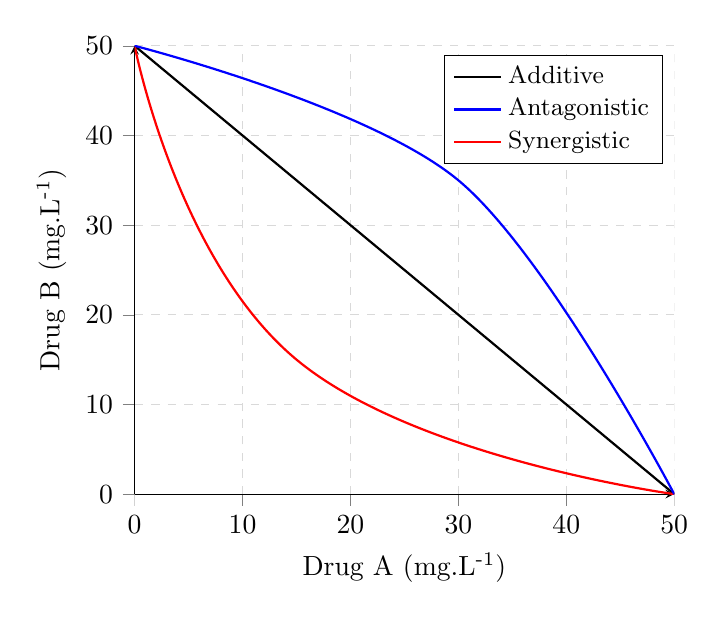
\begin{tikzpicture}

    \begin{axis}[
axis x line=bottom,
  axis y line=left,
	ymin = 0,
	ymax = 50,
	xmin = 0,
xmax = 50,
        grid = major,
        grid style={dashed, gray!30},
	 ylabel near ticks,
	xlabel near ticks,
        xlabel=Drug A (mg.L\textsuperscript{-1}),
        ylabel=Drug B (mg.L\textsuperscript{-1}),
        tick align=outside,
        enlargelimits=false,
legend entries={Normal, Class Ia},
legend style={font=\small, cells={align=left}},
legend cell align={left}]

\addplot[black,thick, domain=0:50] {50-x};
\addlegendentry{Additive};

\draw[red, thick] plot[smooth,tension=0.8] coordinates { (axis cs: 0,50) (axis cs: 15, 15) (axis cs: 50,0)};
\draw[blue, thick] plot[smooth,tension=0.6] coordinates { (axis cs: 0,50)(axis cs: 30, 35) (axis cs: 50,0)};

\addlegendimage{blue, thick};
\addlegendentry{Antagonistic};
 \addlegendimage{red, thick}
\addlegendentry{Synergistic};
\end{axis}

\end{tikzpicture} 
\end{document}